%************************************************
\chapter{Results}\label{ch:Results} 
%************************************************
\section{Training cases}
\subsection{Z score threshold}
Investigating the Z score of probes within regions known to be abnormal suggests a range of Z score thresholds to define probes as abnormal  to investigate (Figure \ref{fig:probeswithinreportedregion}). 
\paragraph*{}
However, reported regions may contain normal probes and whilst sensitivity is favoured over specificity a balance must be found to prevent many false positive calls.

\begin{figure}[h]
\centering
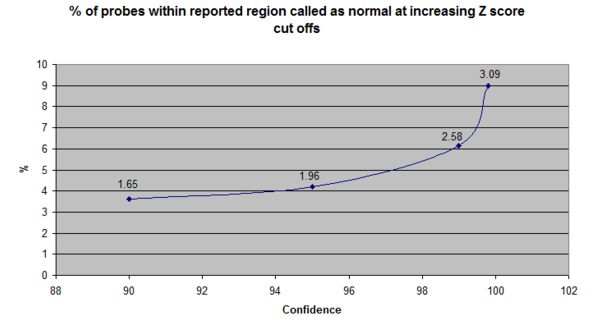
\includegraphics[width=1\linewidth]{./Figures/probeswithinreportedregion}
\caption[The number of probes classified as normal within known regions of CNV at a range of Z score thresholds]{The percentage of probes called as normal within known abnormal regions increases with the Z score threshold. Abnormal regions can include normal probes so even at a Z score threshold of 1.65 over 3\% of probes are called as normal. The Z score is shown above each point}
\label{fig:probeswithinreportedregion}
\end{figure}

\begin{table}[]
\centering
\caption[Calls made in 86 training cases]{A very high number of false positive calls was seen in the 86 training cases using a range of Z score thresholds.}
\label{tab:training_set_calls_86}
\resizebox{\textwidth}{!}{%
\begin{tabular}{@{}lccccccc@{}}
\cmidrule(l){2-8}
\multirow{2}{*}{}                                                                                 & \multicolumn{7}{c}{Z Score}                                                   \\
                                                                                                  & 2.374      & 3         & 3.5      & 3.55     & 3.75     & 4        & 4.25     \\ \cmidrule(l){2-8} 
\% True Positives (n)                                                                             & 92 (79)    & 92 (79)   & 92 (79)  & 92 (79)  & 92 (79)  & 92 (79)  & 88 (76)  \\
\% Arrays with false positives (n)                                                                & 67 (58)    & 45 (39)   & 37 (32)  & 36 (31)  & 33 (28)  & 30 (26)  & 30 (26)  \\
Number of false positive calls                                                                    & 10228        & 7681       & 6177       & 6044       & 5538       & 4944       & 4394       \\
\begin{tabular}[c]{@{}l@{}}Average number of false \\ positive calls per array (max)\end{tabular} & 192.98 (2128) & 225.91 (1733) & 228.78 (1468) & 232.46 (1443) & 240.78 (1351) & 235.43 (1230) & 209.24 (1108)
\end{tabular}%
}
\end{table}


\subsection{Removal of cases with high false positive calls}
A range of Z score thresholds were applied, starting at $\pm  $ 2.374,  defining abnormal probes as the upper 1\% and lower 1\% of the reference range, and increasing up to 4.25 (Table \ref{tab:training_set_calls_86}).
\paragraph*{}
At the lowest Z score threshold (2.374) the false negative rate was 8\% with 67\% of cases containing a false positive call.
\paragraph*{}
The same Z score threshold resulted in 10228 false positive calls, of which 94\% came from just five arrays (range 1612-2128). The average number of false positive calls in the other 81 arrays was 10.8 (max 104) (Table \ref{tab:training_set_calls}).
\paragraph*{}
Visual inspection of the array traces and the raw data from these 5 arrays gave no indication why so many false positives calls were made or how this could be mediated/predicted. Therefore these five arrays were considered a different population and excluded from further analysis.
\subsection{Comparison of true positive and false positive calls}
\begin{table}[]
\centering
\caption[Calls made in 81 training cases after removal of outliers]{The calls made in 81 training cases using a range of Z score thresholds. The true positive call was missed in at least 5 cases across all thresholds, with a false positive call made in at least 1 in 4 cases. The number of false positive calls, and the average number of calls made decreased as the Z score threshold increased.}
\label{tab:training_set_calls}
\resizebox{\textwidth}{!}{%
\begin{tabular}{@{}lccccccc@{}}
\cmidrule(l){2-8}
\multirow{2}{*}{}                                                                                 & \multicolumn{7}{c}{Z Score}                                                   \\
                                                                                                  & 2.374      & 3         & 3.5      & 3.55     & 3.75     & 4        & 4.25     \\ \cmidrule(l){2-8} 
\% True Positives (n)                                                                             & 94 (76)    & 94 (76)   & 94 (76)  & 94 (76)  & 94 (76)  & 94 (76)  & 90 (73)  \\
\% Arrays with false positives (n)                                                                & 65 (53)    & 42 (34)   & 33 (27)  & 32 (26)  & 28 (23)  & 26 (21)  & 26 (21)  \\
Number of false positive calls                                                                    & 571        & 114       & 50       & 48       & 41       & 35       & 31       \\
\begin{tabular}[c]{@{}l@{}}Average number of false \\ positive calls per array (max)\end{tabular} & 10.8 (104) & 3.35 (20) & 1.85 (7) & 1.84 (7) & 1.78 (7) & 1.66 (6) & 1.48 (5)
\end{tabular}%
}
\end{table}
\paragraph*{}
The remaining 81 arrays show that at least one call was detected within the abnormal region in 94\% of cases with a Z score up to 4 (Table \ref{tab:training_set_calls}).
\\
Using a Z score of 2.374 nearly 2 in 3 arrays had a false positive call. A Z score threshold of 4 reduced the frequency of false positive calls to 1 in 4 arrays, with an average 1.66 and maximum 6 false positive calls per array.

\subsubsection{Number of probes within a call}
The length of false positive calls are shorter than true positive calls. Increasing the minimum number of probes within a call would remove these false positive calls but would also remove true positive calls and fail to meet the functional requirement that a call is a minimum of 3 consecutive probes (Figure \ref{fig:nprobes_2_374}).

\begin{figure}[h]
\centering
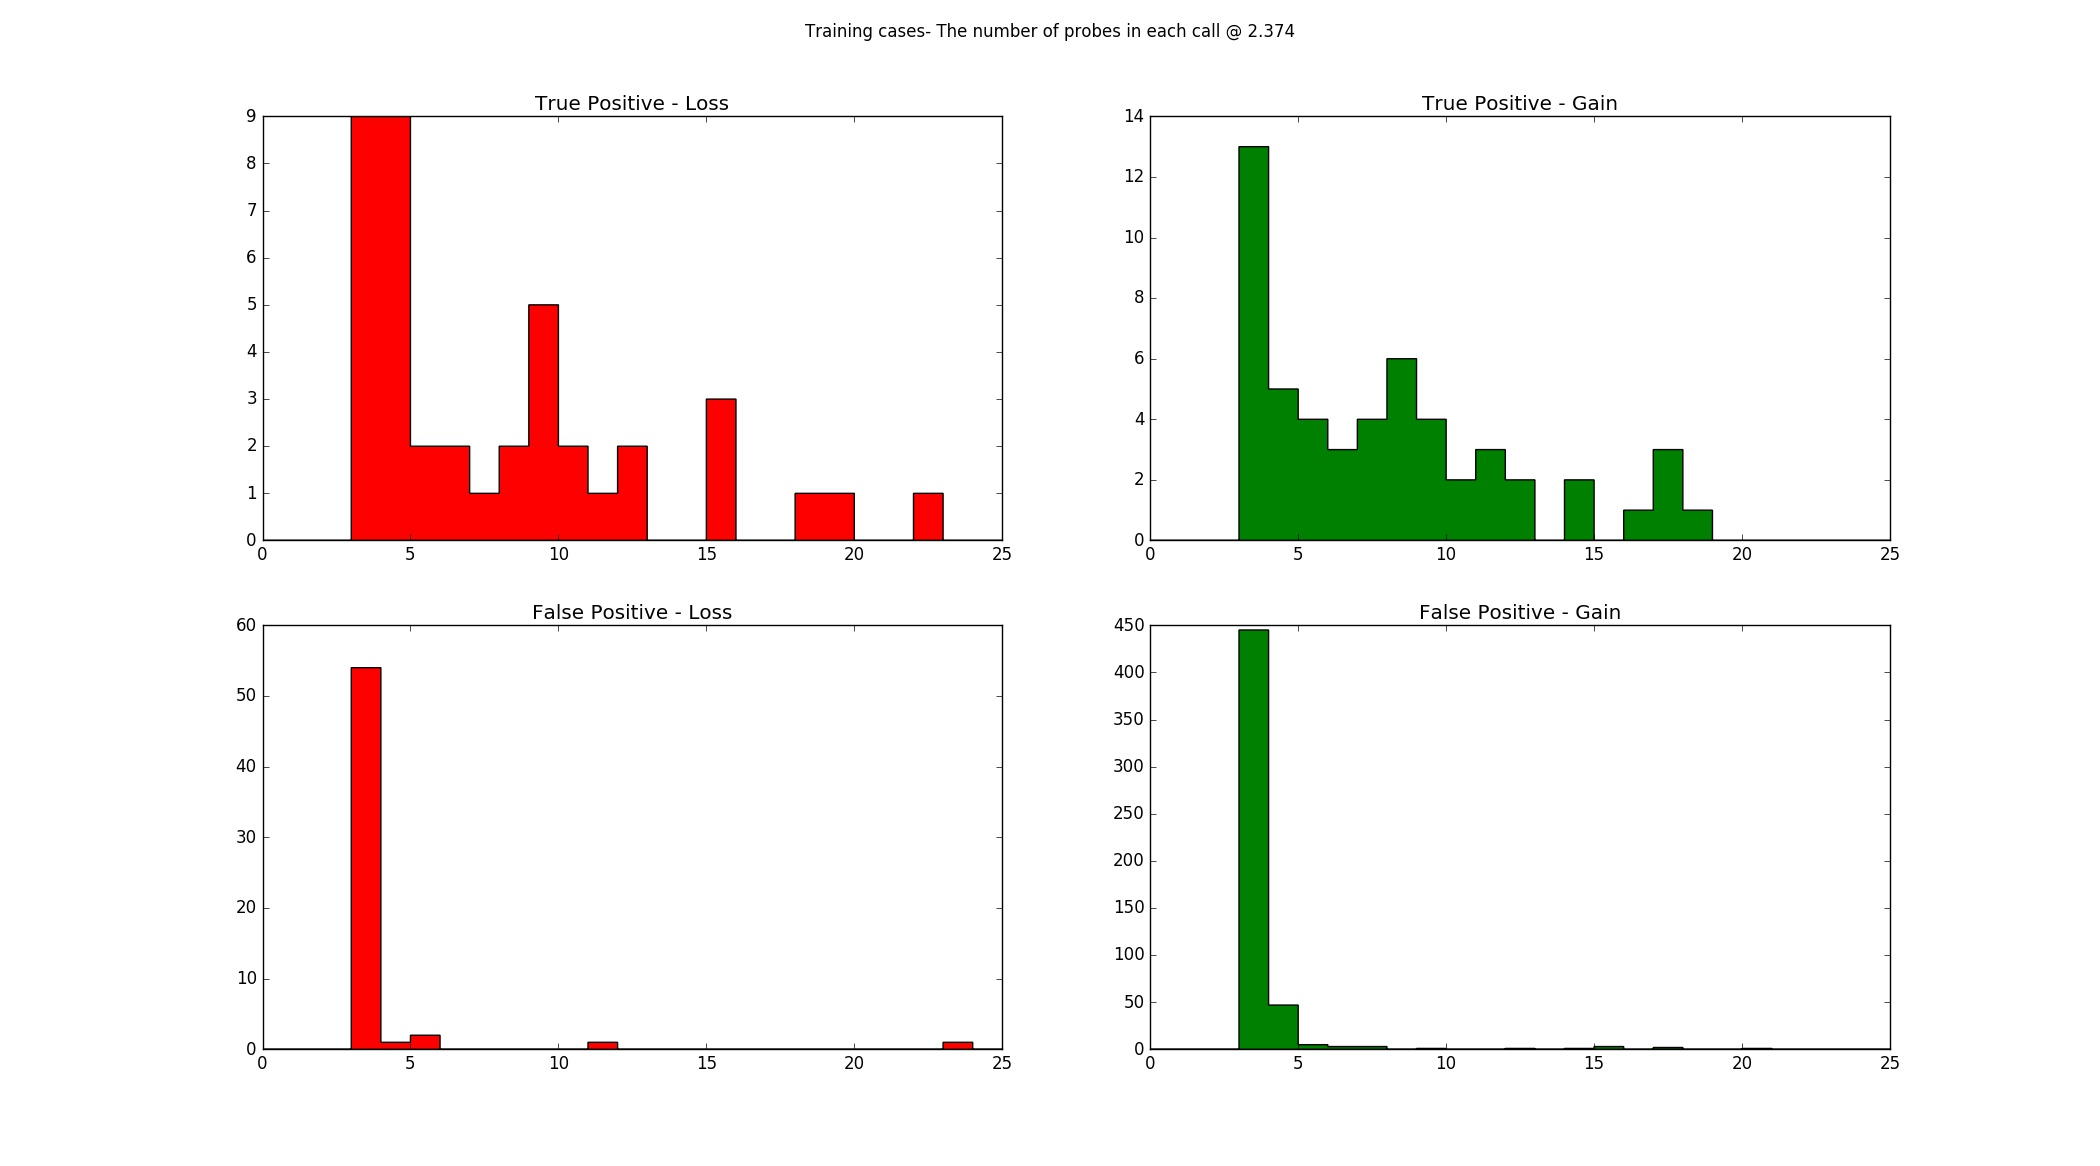
\includegraphics[width=\linewidth]{./Figures/nprobes_2_374}
\caption{Training cases: False positive calls are smaller than true positive calls.}
\label{fig:nprobes_2_374}
\end{figure}

\subsubsection{Difference between true and false positive Z scores using a threshold of 2.374}
Alternatively increasing the Z score threshold to above the lowest scoring probe in abnormal regions may prevent the region being called \ref{fig:consecutiveprobeanalysis}.
\paragraph*{}
Examining the minimum (Figure \ref{fig:lowest_2_374}) and average (Figure \ref{fig:average_2_374}) Z scores for each true and false positive calls show that the two populations are not disparate therefore increasing the Z score threshold may also remove true positives. 
\begin{figure}[h]
\centering
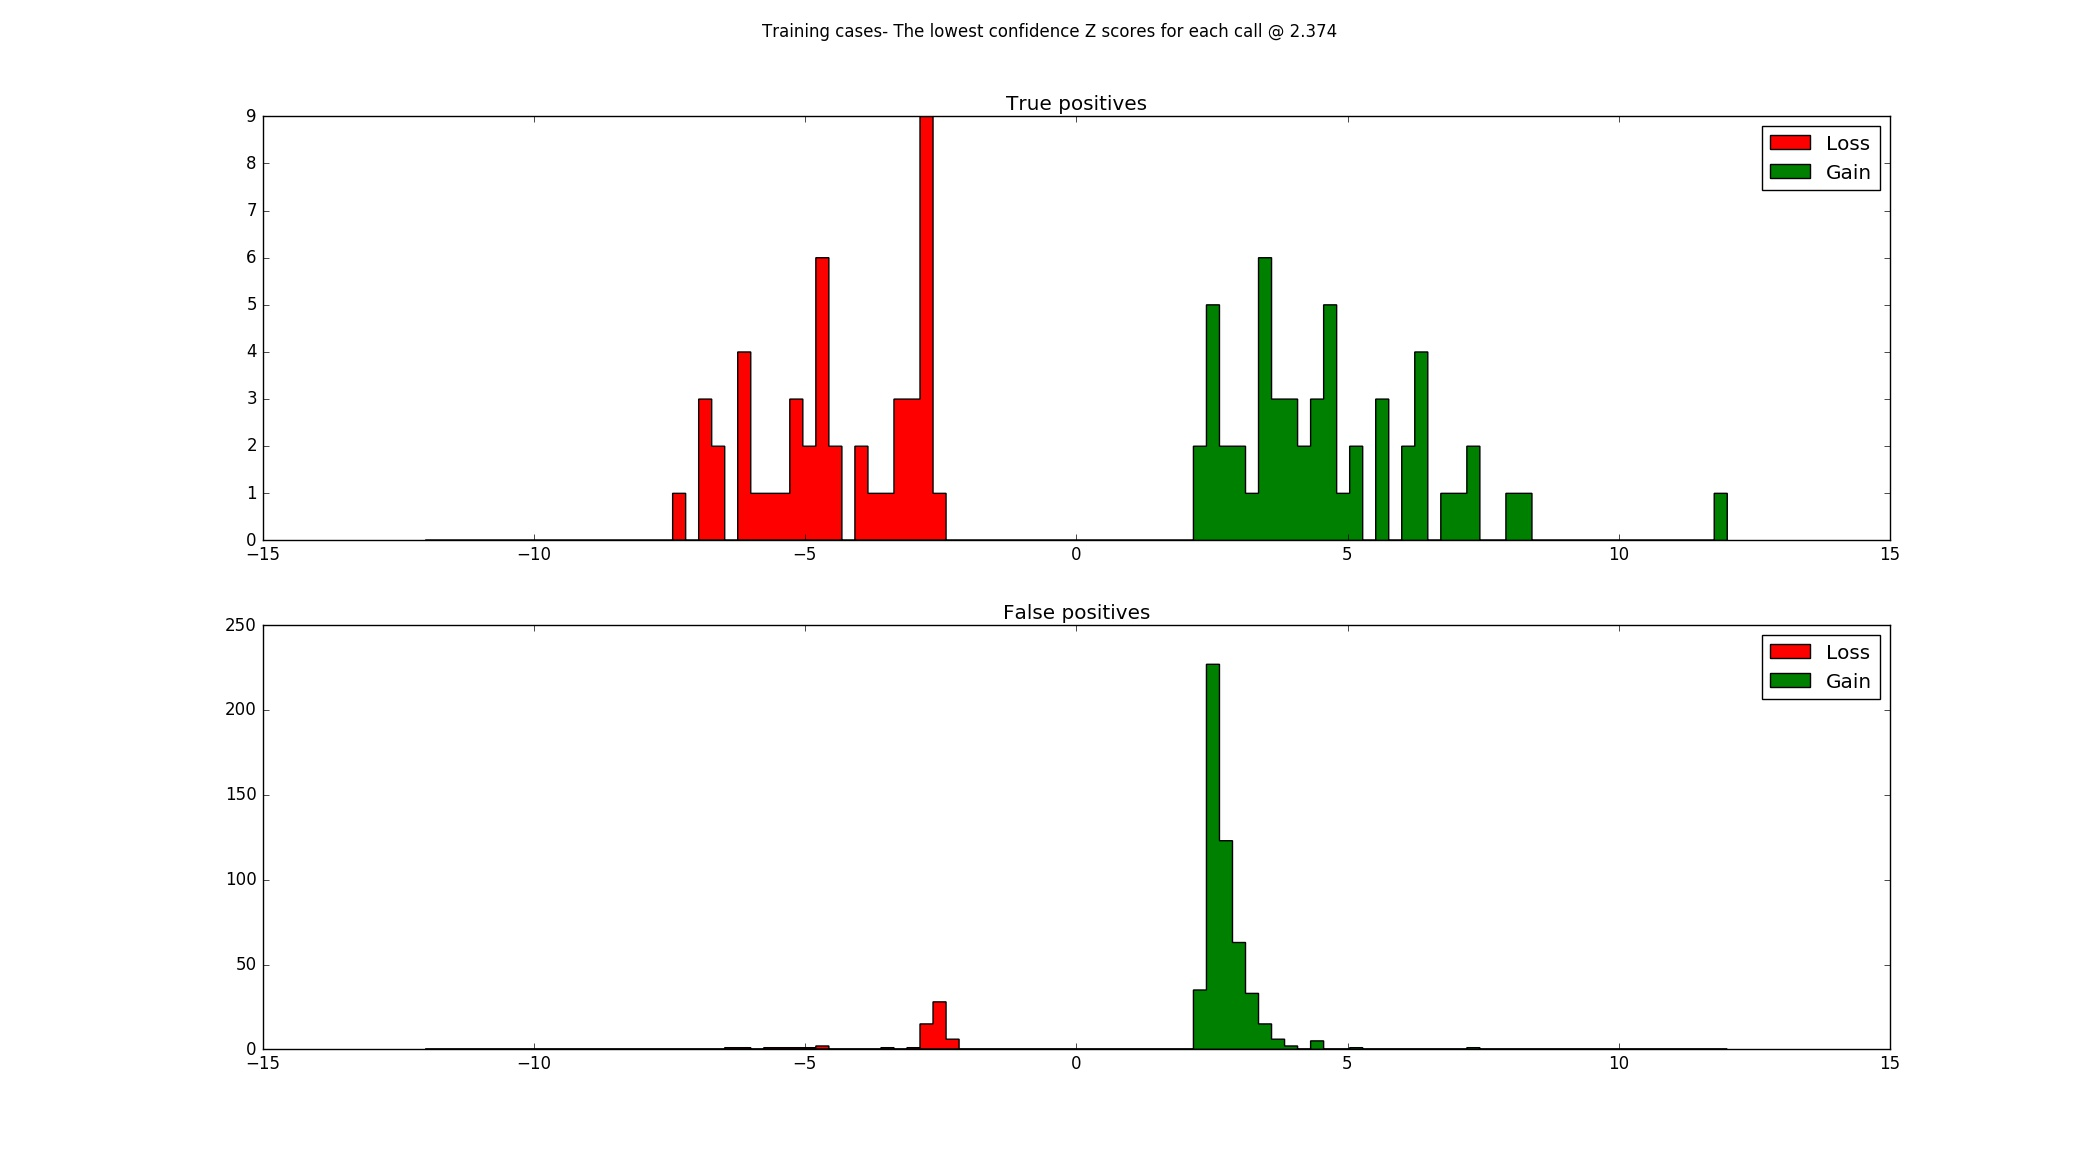
\includegraphics[width=1\linewidth]{./Figures/lowest_2_374}
\caption[Training cases: The lowest confidence Z score within each call at a threshold of 2.374]{Training cases: The lowest confidence Z score within each call at a threshold of 2.374. There is an overlap between the confidence of the lowest probe within true and false positive calls}
\label{fig:lowest_2_374}
\end{figure}

\begin{figure}[h]
\centering
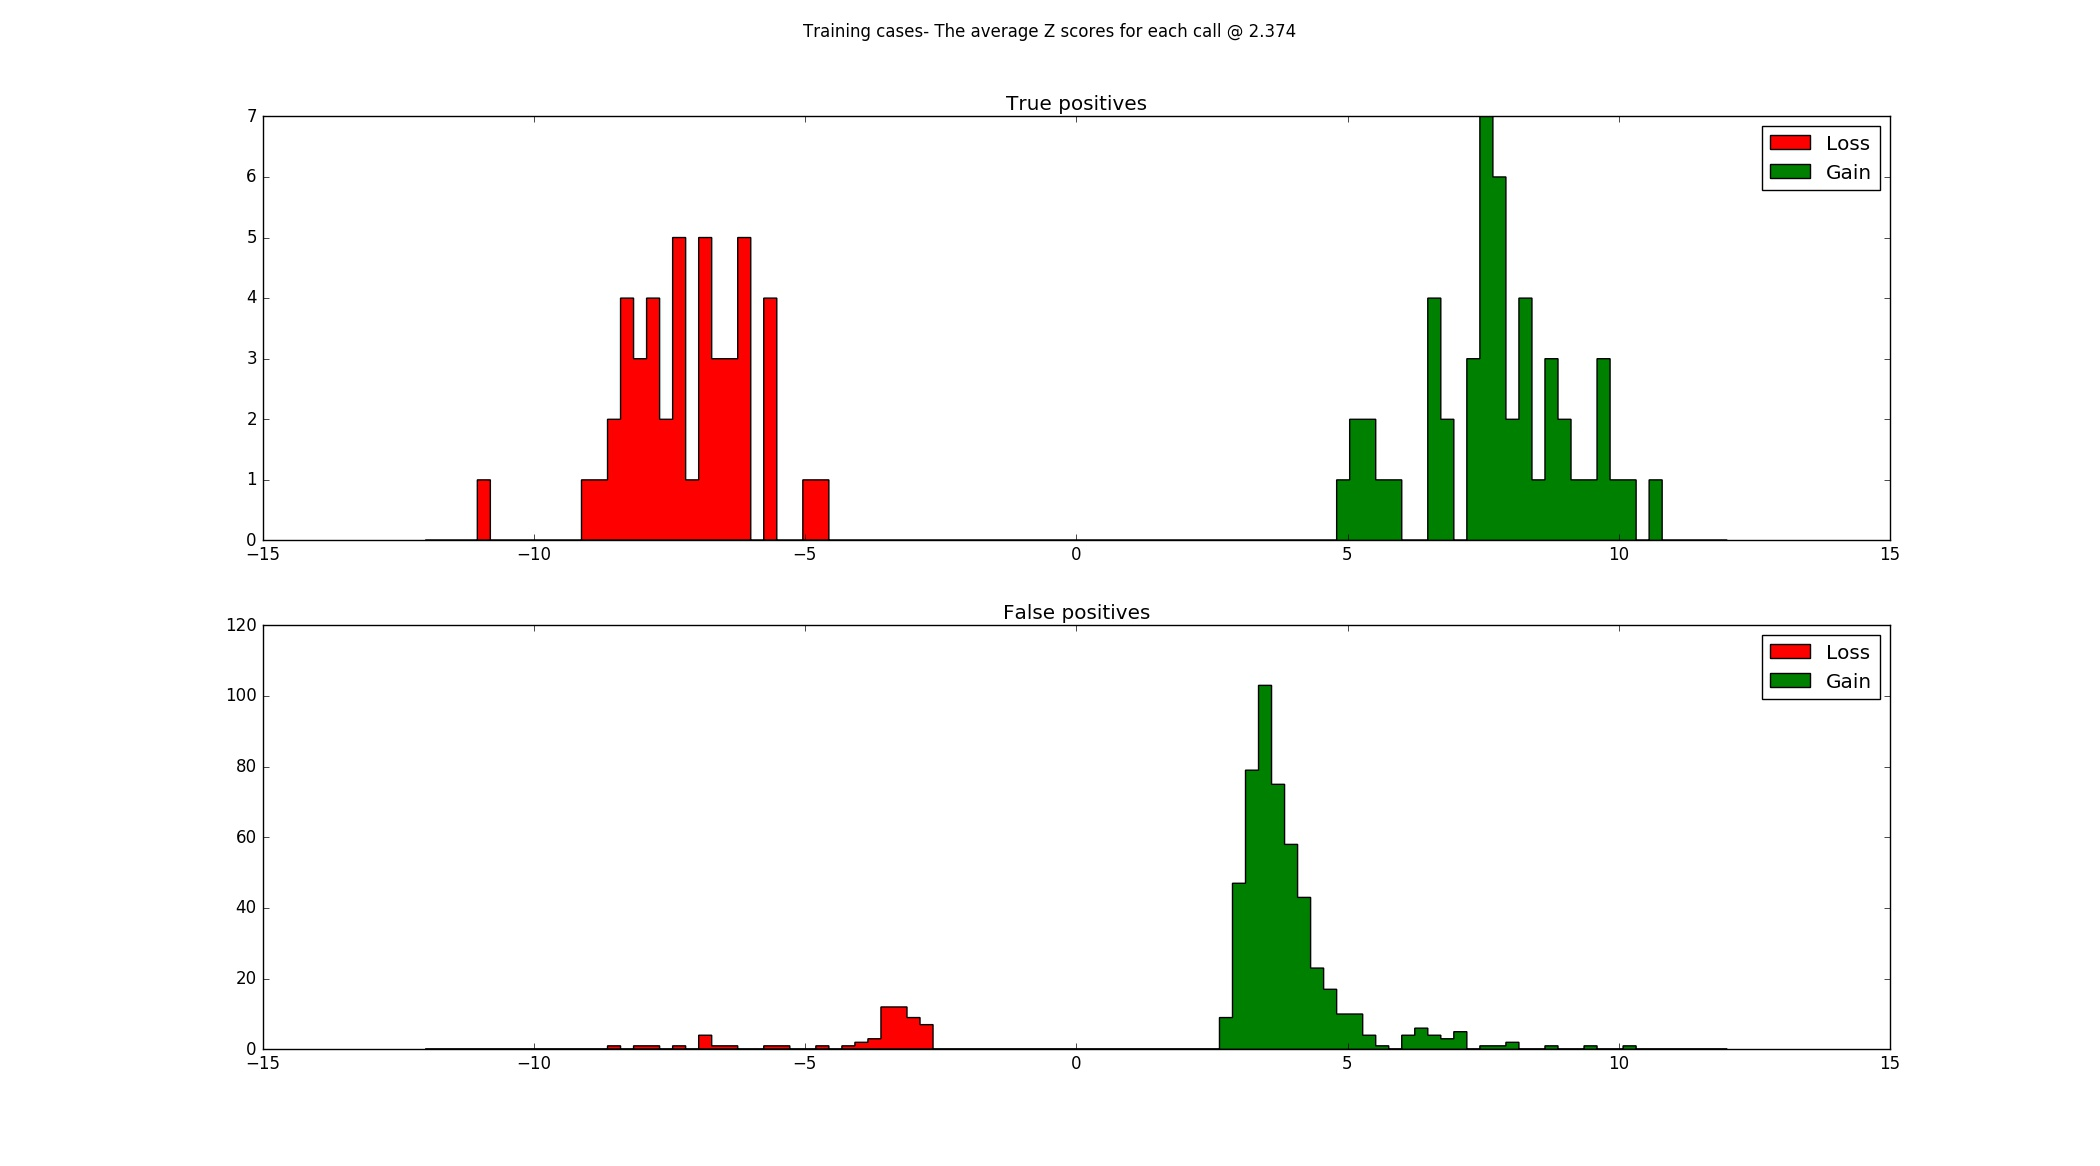
\includegraphics[width=1\linewidth]{./Figures/average_2_374}
\caption[Training cases: The average Z score of probes within calls at a threshold of 2.374]{Training cases: The average Z score of probes within calls at a threshold of 2.374. The average Z score of true positive calls are further from the mean than the average Z score of false positive calls.}
\label{fig:average_2_374}
\end{figure}

\paragraph*{}
However the increased number of probes within a true positive region (Figure \ref{fig:nprobes_2_374}) and the higher average Z score (Figure \ref{fig:average_2_374}) may mean the true positive regions remain.

\subsubsection{Difference between true and false positive Z scores using a threshold of 3.55}
Increasing the Z score threshold to 3.55 showed that the lowest confidence Z scores in remaining false positive calls were similar to that of true positives (Figure \ref{fig:lowest_3_55}).

\begin{figure}[h]
\centering
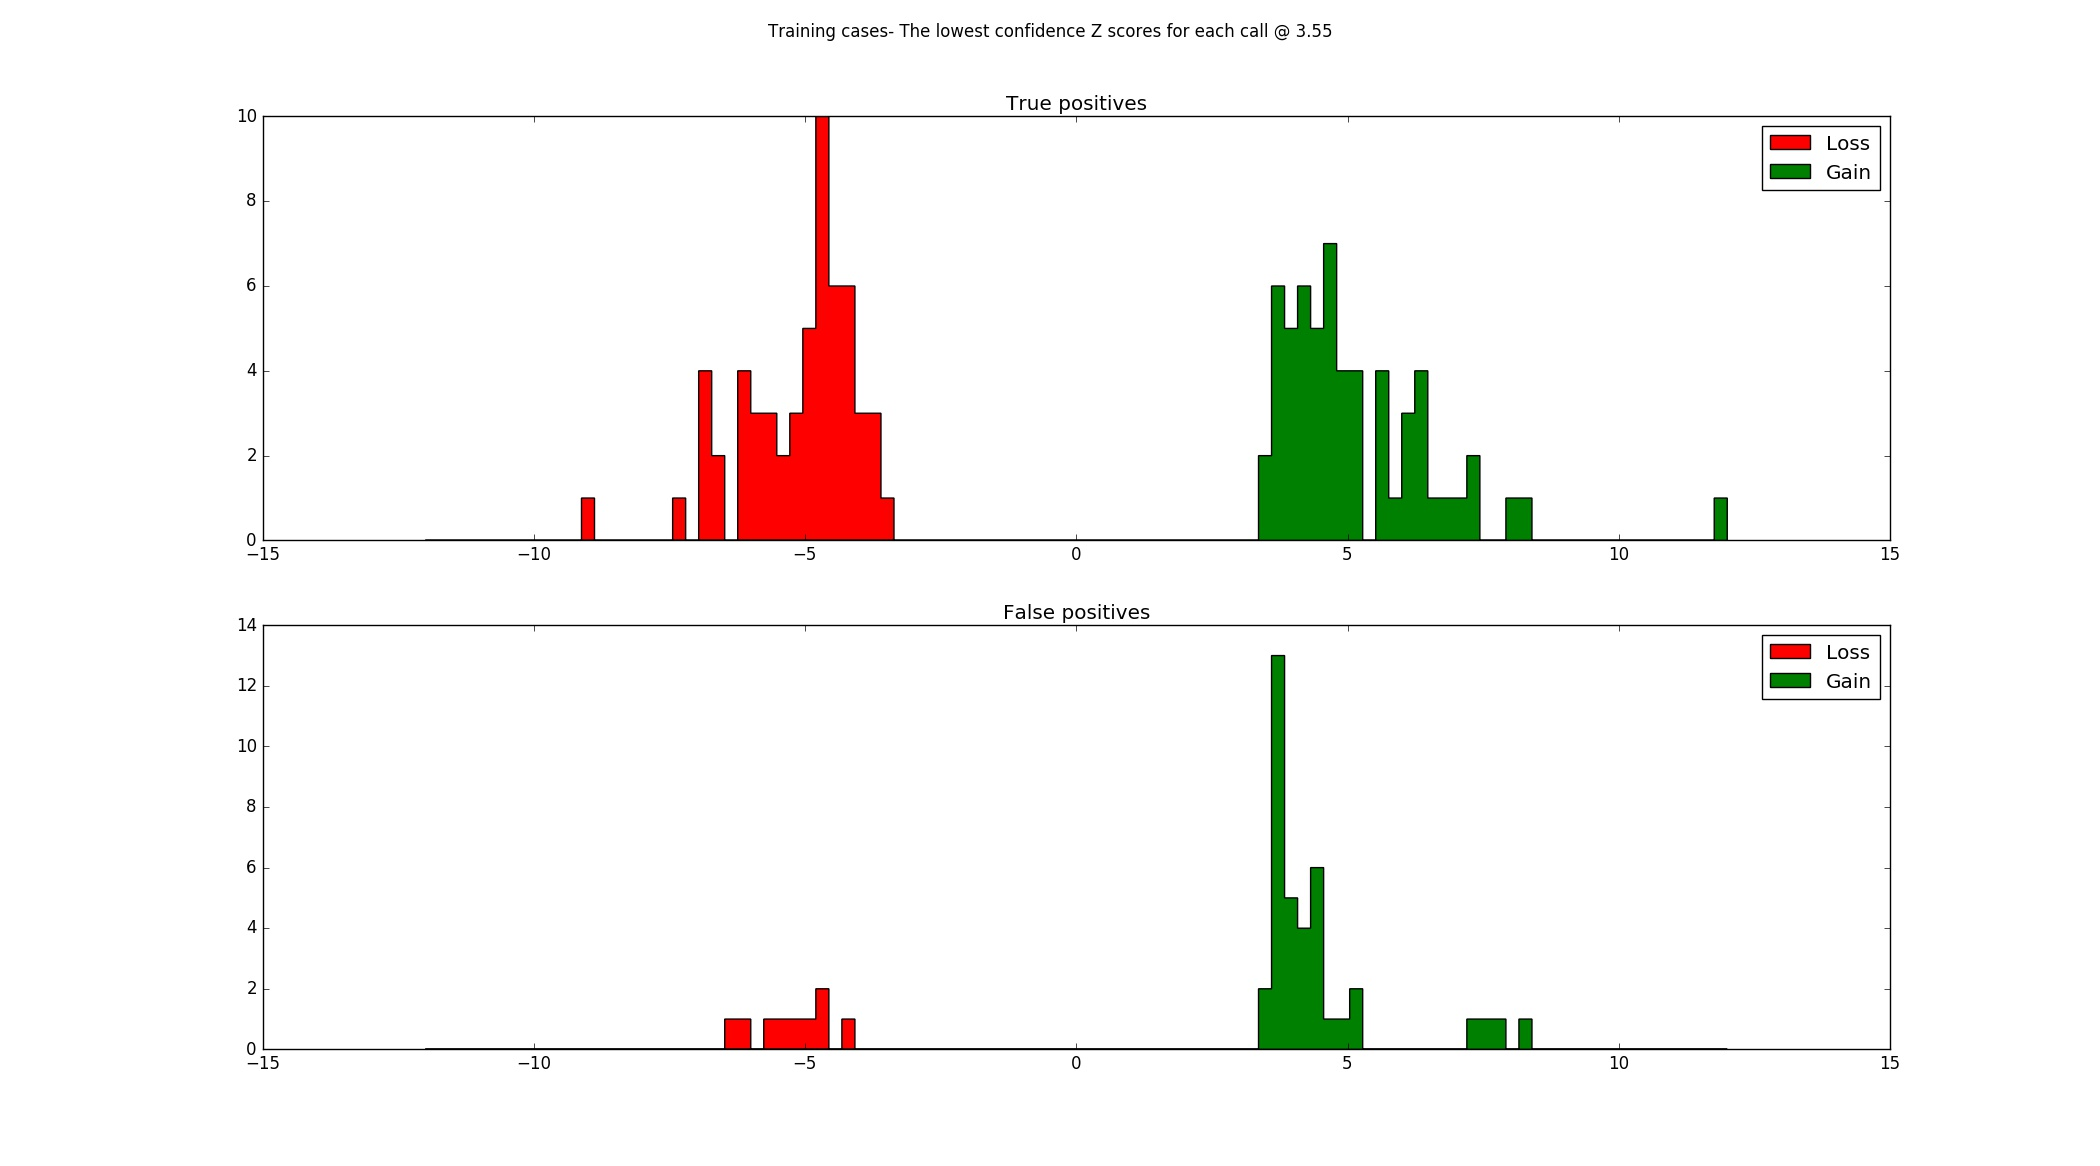
\includegraphics[width=1\linewidth]{./Figures/lowest_3_55}
\caption[Training cases: The lowest confidence probe within calls at a threshold of 3.55]{Training cases: At a threshold of 3.55 the lowest confidence probes within true and false calls are very similar}
\label{fig:lowest_3_55}
\end{figure}

\paragraph*{}
Similarly the distribution of average Z scores were very similar between true and false positives calls (Figure \ref{fig:average_3_55}).

\begin{figure}[h]
\centering
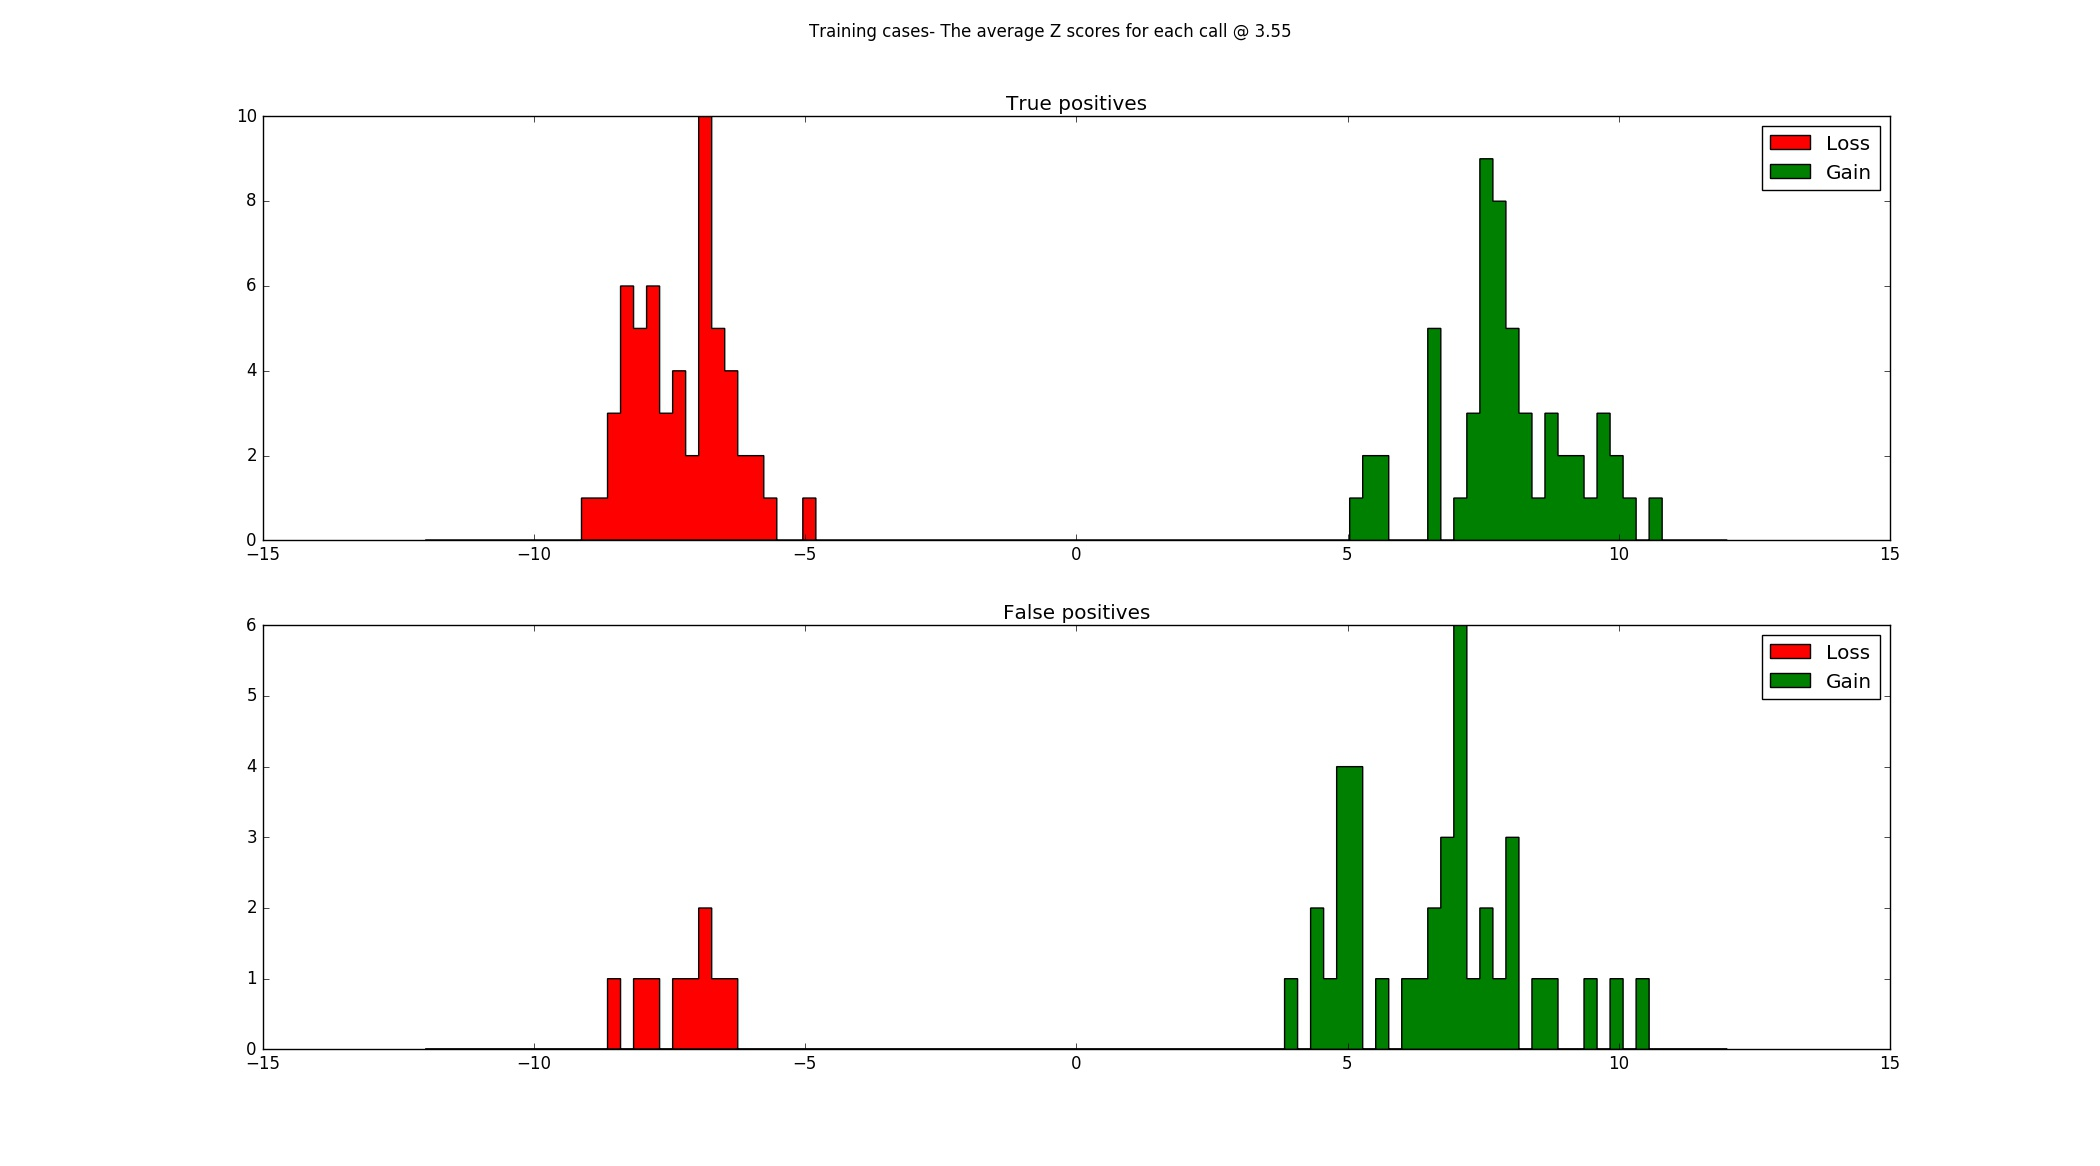
\includegraphics[width=1\linewidth]{./Figures/average_3_55}
\caption[Training cases:Average Z scores for calls made with a threshold of 3.55]{Training cases: The average Z score for probes within true and false positive calls with a threshold of 3.55 are very similar.}
\label{fig:average_3_55}
\end{figure}

\subsubsection{Suitability of reference range}
There were no recurring false positives calls to suggest the reference ranges were unsuitable.

\section{Test Cases}
The training cases are not truly representative of an array where both hybridisation partners have the same CNV. Cy3 and Cy5 dyes are incorporated with varying efficacy so the reference value will vary. When calculating the Z score for these cases comparing the signal intensity of one dye to the reference value of the other dye may introduce error.
\paragraph*{}
The same thresholds were applied to 69 test cases \ref{tab:testset_calls}. 

\begin{figure}
\centering
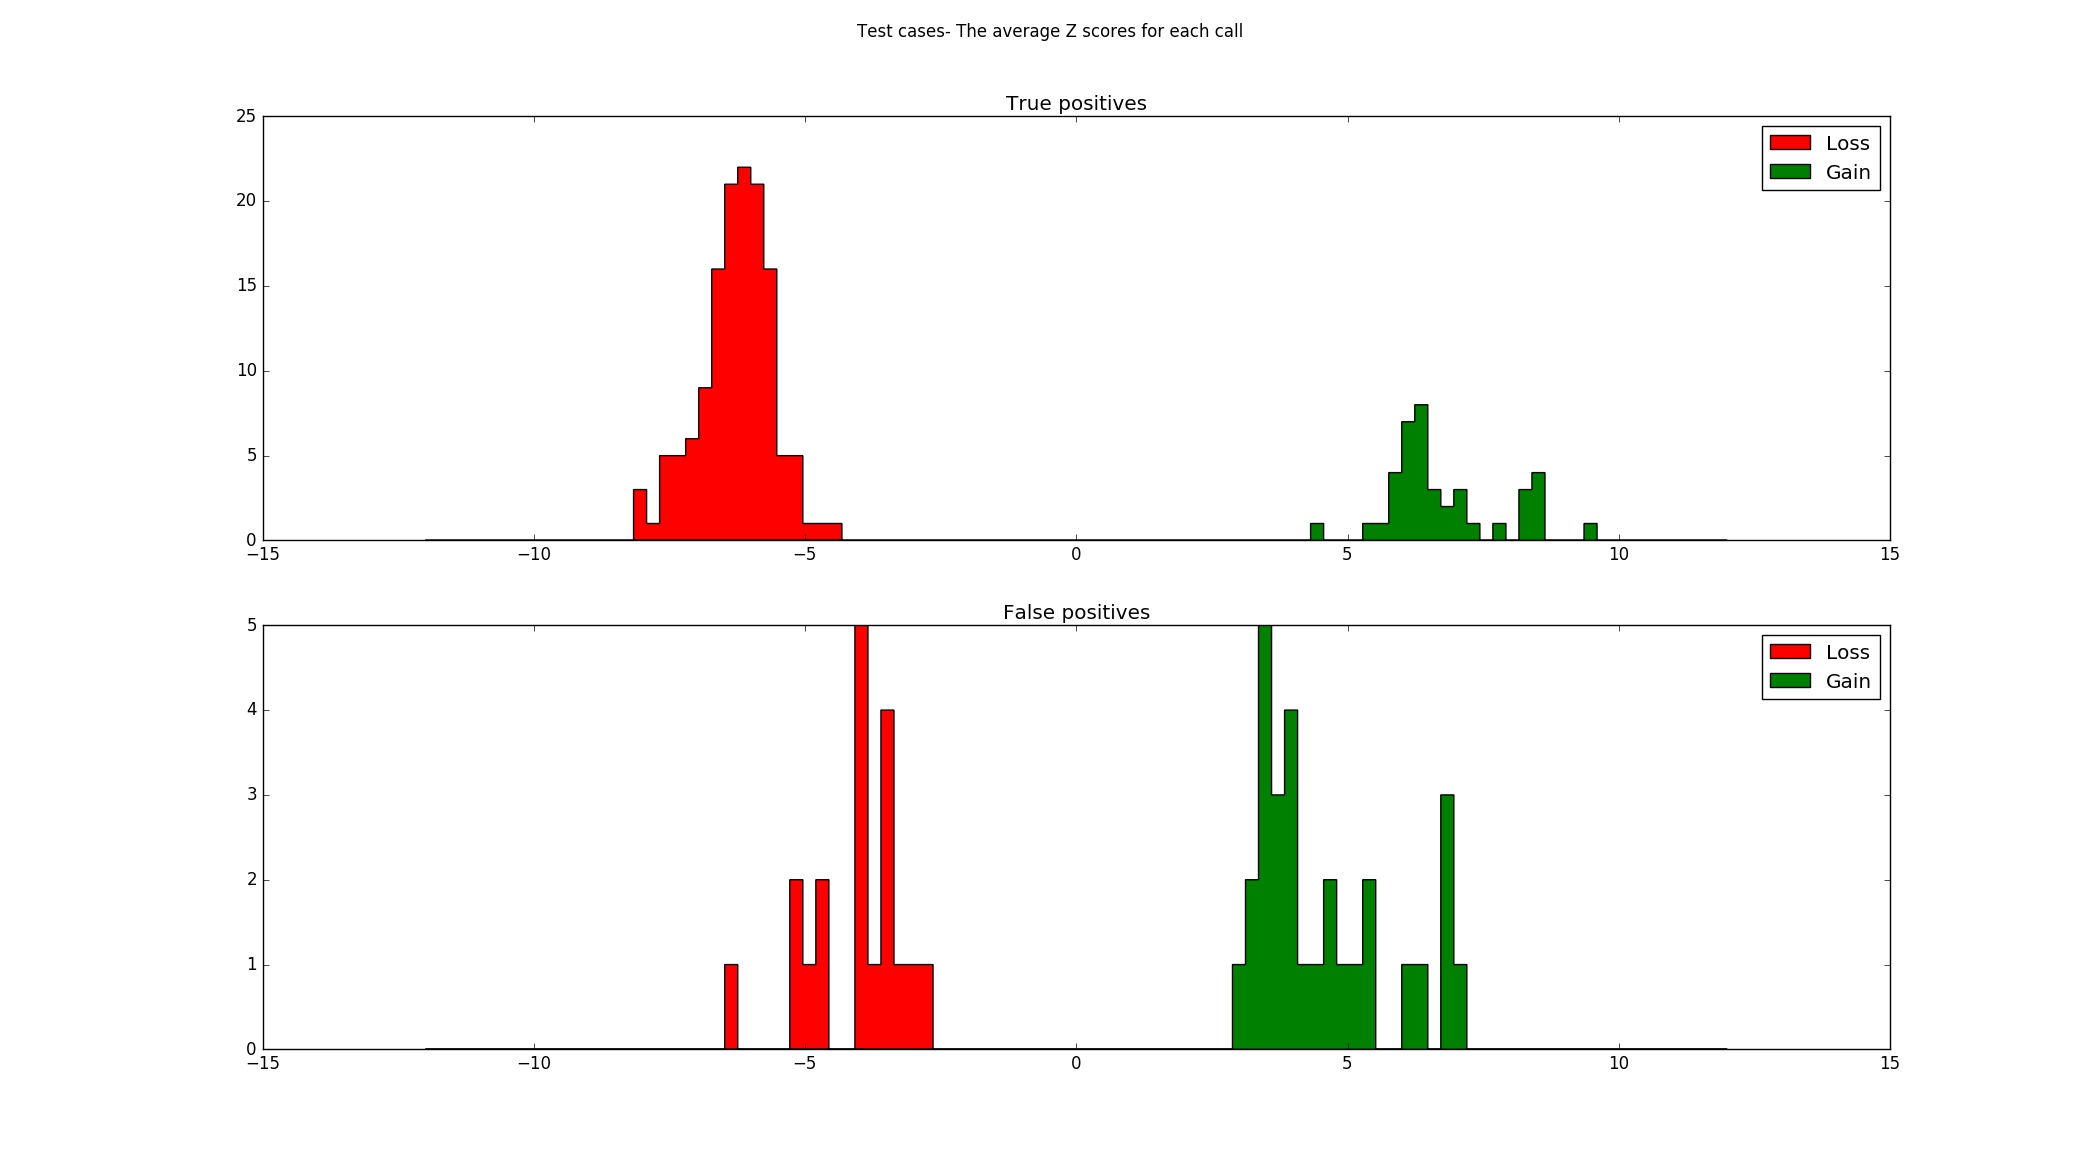
\includegraphics[width=1\linewidth]{./Figures/testcasesaverageconfidenceZscore}
\caption[Test cases: The average Z score at a threshold of 2.374]{Test cases: The average Z score in true positive calls made at a threshold of 2.374 are more significant in true positive calls than false positive calls however there is overlap between the two groups}
\label{fig:testcasesaverageconfidenceZscore}
\end{figure}

\begin{figure}
\centering
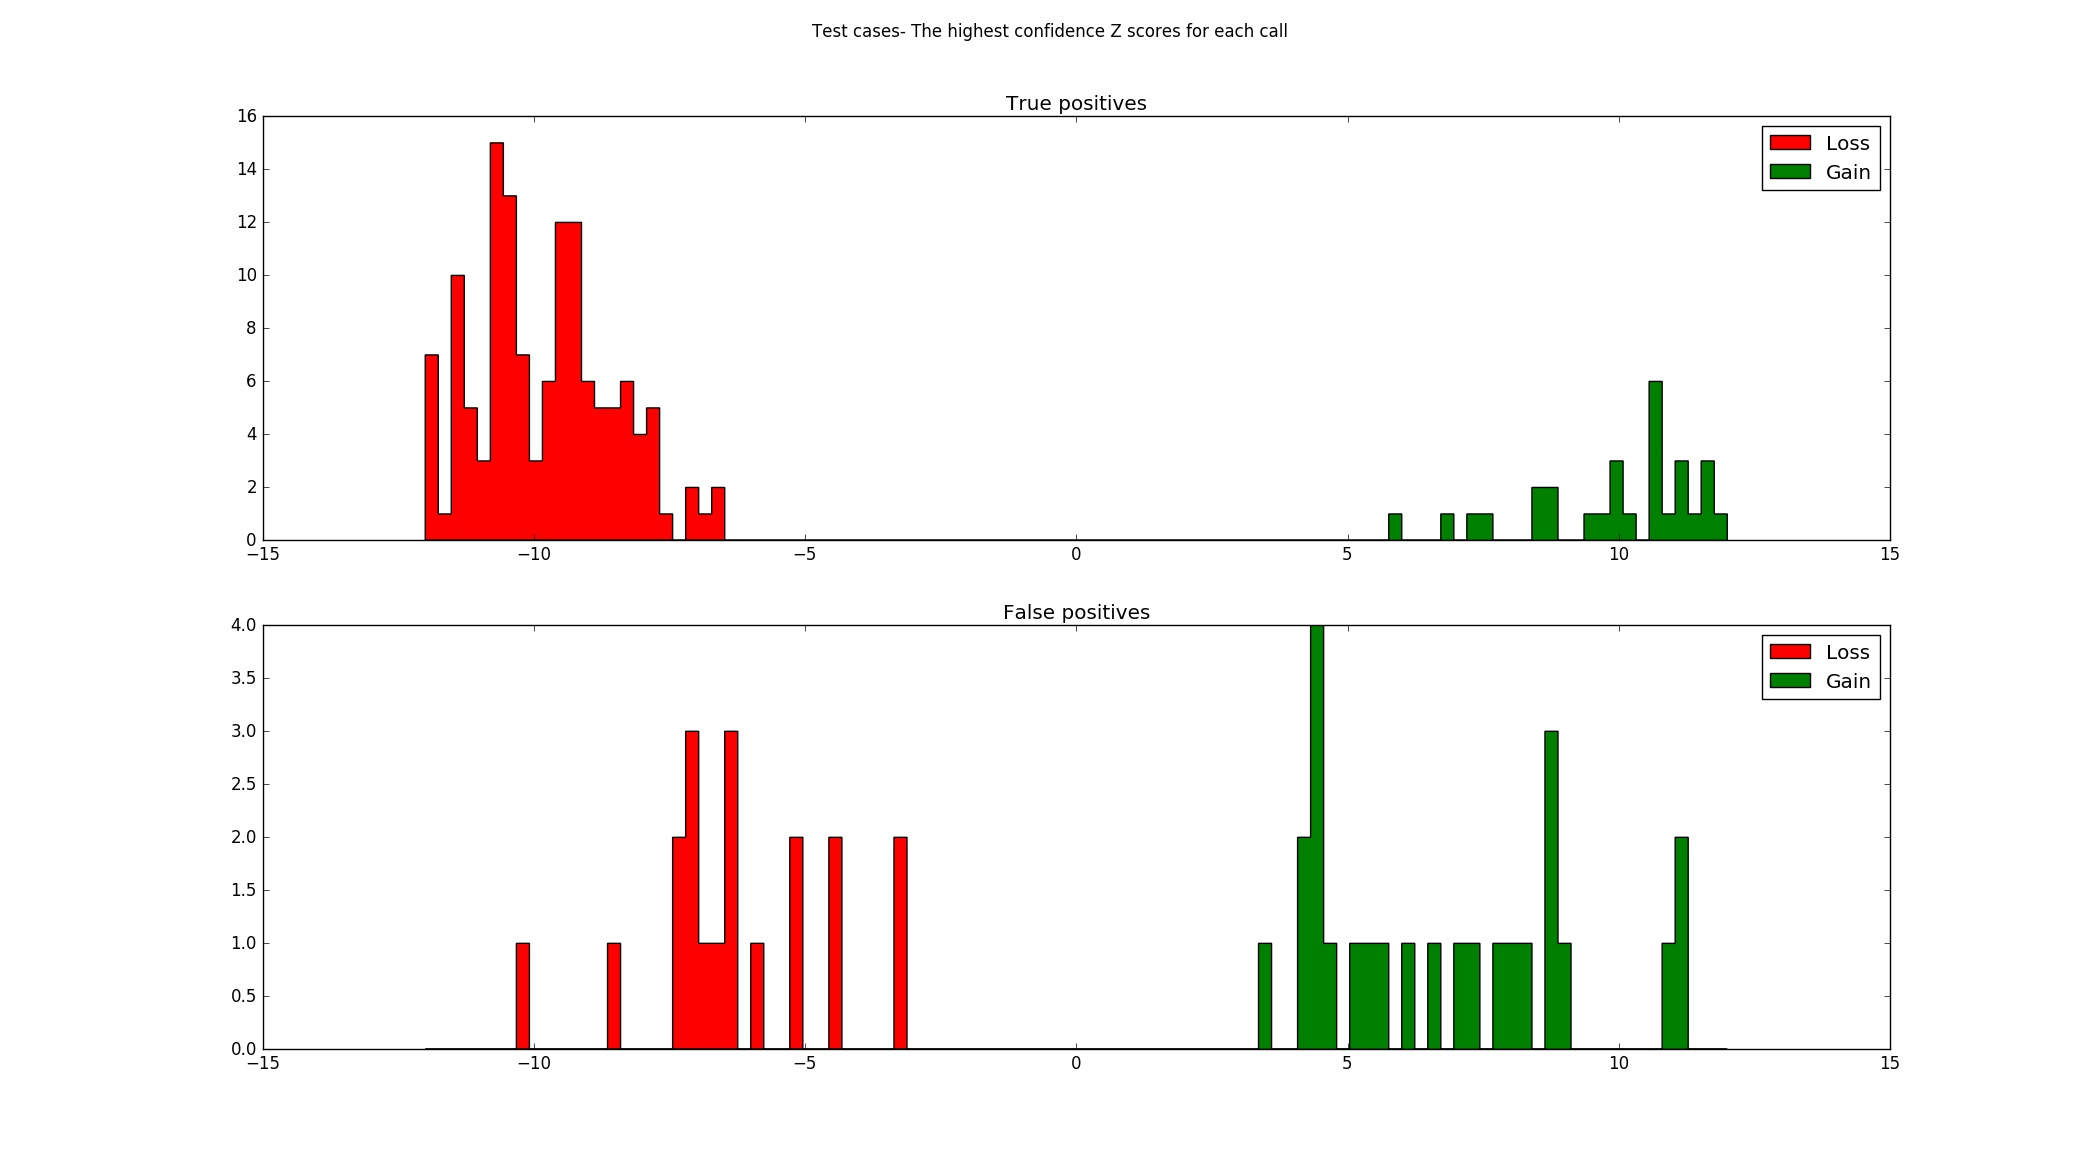
\includegraphics[width=1\linewidth]{./Figures/testcaseshighestconfidenceZscore}
\caption[Test cases: The highest confidence probe within calls made at a threshold of 2.374]{Test cases: At a Z score threshold of 2.374 there is an overlap between the highest confidence probe within true and false positive calls.}
\label{fig:testcaseshighestconfidenceZscore}
\end{figure}

\begin{figure}
\centering
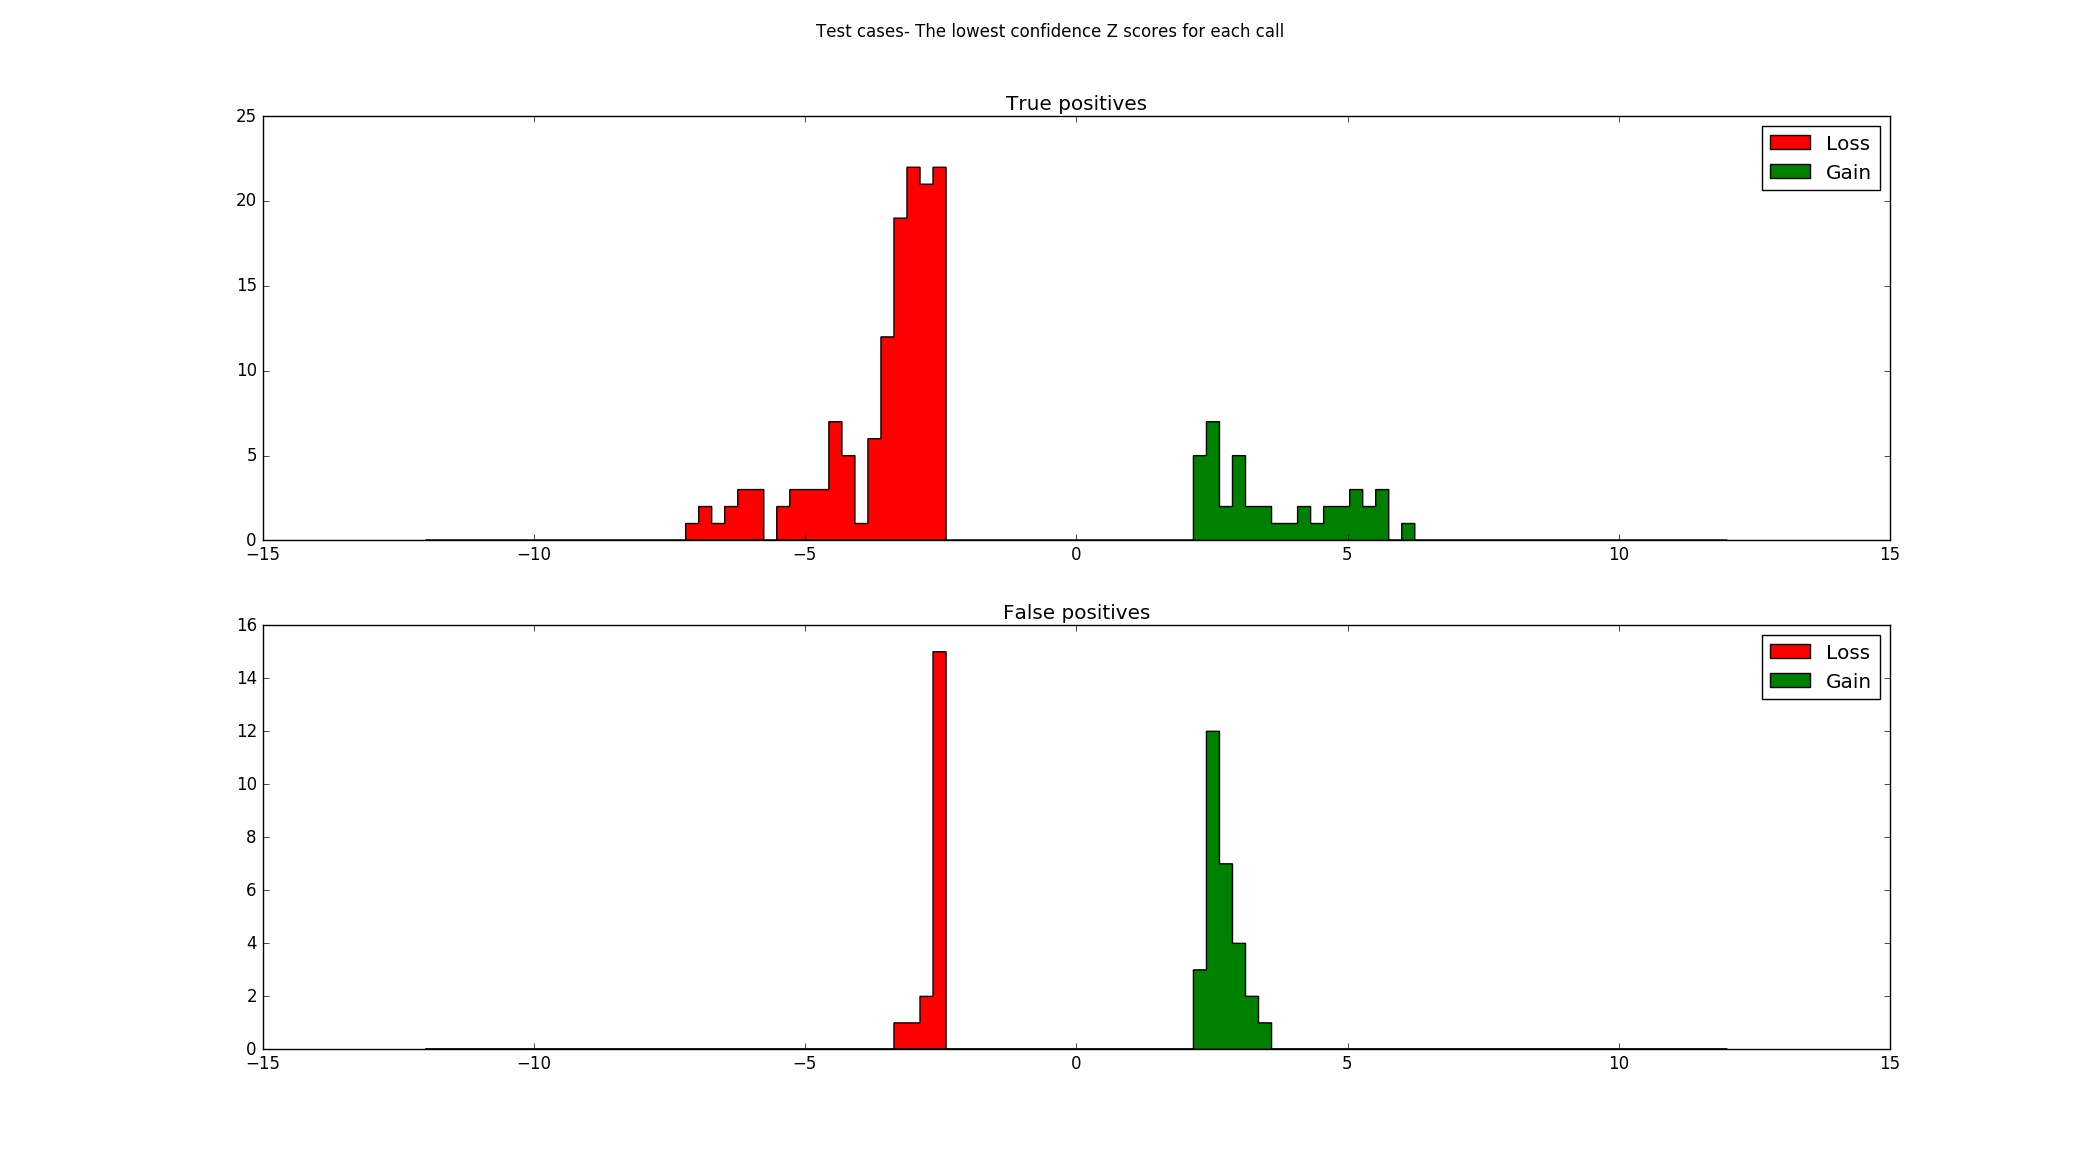
\includegraphics[width=1\linewidth]{./Figures/testcaseslowestconfidenceZscore}
\caption[Test cases: The lowest confidence probe within calls at a threshold of 2.374]{Test cases: There is overlap between the lowest confidence probe within true and false positive calls made at a threshold of 2.374}
\label{fig:testcaseslowestconfidenceZscore}
\end{figure}

\begin{figure}
\centering
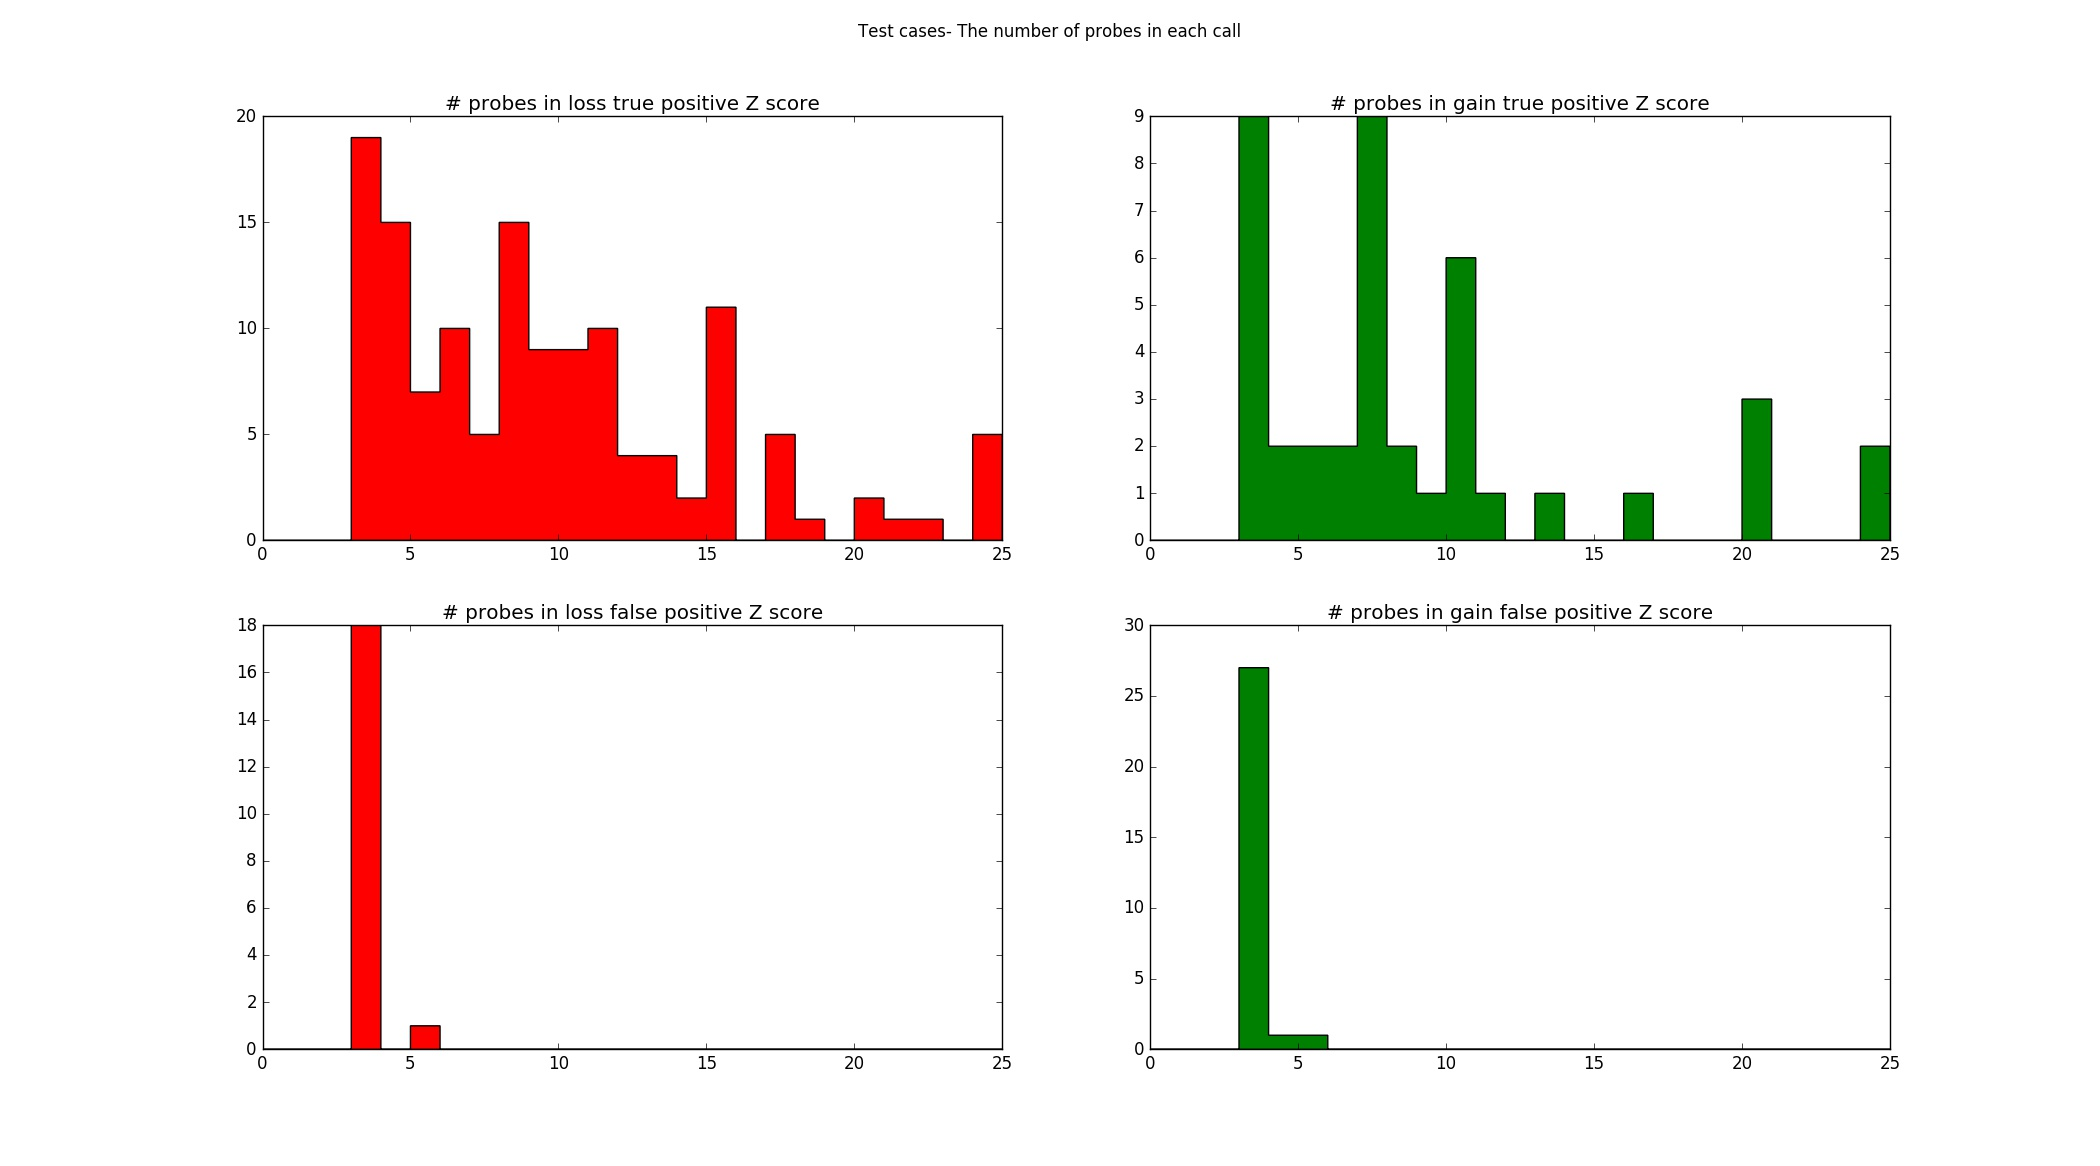
\includegraphics[width=1\linewidth]{./Figures/testcasesprobecount}
\caption[Test cases:  The number of probes within calls made at a threshold of 2.374]{Test cases: At a threshold 2.374 true positive calls contain more probes than false positive calls.}
\label{fig:testcasesprobecount}
\end{figure}

\paragraph*{}
There were no recurring false positive calls.

\subsection{A greater sensitivity was seen using more representative feature extraction files}
There was 100\% sensitivity using a Z score below 4 and there were no false positive calls using a Z score above 3.55 \ref{tab:testset_calls}. 


\begin{table}[]
\centering
\caption[Test cases: Calls made at a range of thresholds]{Test cases: A call was made in the expected CNV region in all cases with a threshold below 4. There were no false positive calls made with a threshold above 3.55}
\label{tab:testcasetable}
\resizebox{\textwidth}{!}{%
\begin{tabular}{@{}lccccccc@{}}
\cmidrule(l){2-8}
\multirow{2}{*}{}                    & \multicolumn{7}{c}{Z score}                                               \\ \cmidrule(l){2-8} 
                                     & 2.375    & 3        & 3.5      & 3.55     & 3.75     & 4        & 4.25    \\ \cmidrule(l){2-8} 
\% True Positive arrays (n)          & 100 (69) & 100 (69) & 100 (69) & 100 (69) & 100 (69) & 100 (69) & 97 (67) \\
\% Arrays with false positives (n)   & 13 (9)   & 8.7 (6)  & 1.4 (1)  & 0        & 0        & 0        & 0       \\
Number of false positive calls (max) & 48 (28)  & 9 (3)    & 1 (1)    & 0        & 0        & 0        & 0      
\end{tabular}%
}
\end{table}

\subsection{Proportion of CNV regions covered by calls}
As shown in Figure \ref{fig:testcasestrueposcoverage} with the exception of 8 arrays with the 750 probe deletion on chromosome 22 (see Table \ref{tab:testset_calls}) at least 25\% of the probes were included within a call, with an average of 66\% of the CNV included within a call.

\begin{figure}
\centering
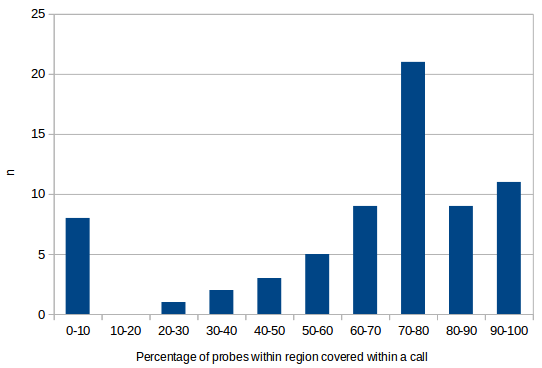
\includegraphics[width=1\linewidth]{./Figures/testcasestrueposcoverage}
\caption[Test cases: the proportion of probes within reported CNV included by a call at a threshold of 3.55]{The proportion of probes within reported CNV included by a call at a threshold of 3.55.}
\label{fig:testcasestrueposcoverage}
\end{figure}


\section{Prospective cases}
121 routine arrays were processed. The expected results are unknown but the number of calls is indicative of the number of calls required to be assessed during analysis.
\paragraph*{}
Using the Z score threshold of 2.374 there were a significant number of calls, with more than 1 in 3 cases having calls to investigate. A threshold of 3.55 resulted in a call in at least 1 in 9 arrays (Table \ref{tab:prospectivecasecalls}).
\paragraph*{}
The maximum number of calls in a single array is quite high, with one array having 199 calls at a threshold of 3.55.

\begin{table}[]
\centering
\caption[Prospective cases: The prevalence of calls]{Prospective Cases: The proportion of the 121 arrays where a call has been made, and the total number of calls made across a range of thresholds. At a threshold of 3.55 12\% of arrays contain a call. Across these 14 cases there are 246 calls, of which 119 is made in a single case.}
\label{tab:prospectivecasecalls}
\resizebox{\textwidth}{!}{%
\begin{tabular}{|l|l|l|}
\hline
Z score & \begin{tabular}[c]{@{}l@{}}\% of arrays with a call\\ (n)\end{tabular} & \begin{tabular}[c]{@{}l@{}}Total number of calls\\ (max calls in a single array)\end{tabular} \\ \hline
2.374   & 37 (45)                                                                           & 1760 (555)                                                                                   \\ \hline
3       & 16 (19)                                                                           & 591 (219)                                                                                    \\ \hline
3.55    & 12 (14)                                                                           & 246 (119)                                                                                    \\ \hline
3.75    & 12(14)                                                                           & 186 (98)                                                                                     \\ \hline
4       & 10 (12)                                                                          & 125 (66)                                                                                     \\ \hline
4.25    & 7 (9)                                                                           & 90 (50)                                                                                      \\ \hline
\end{tabular}%
}
\end{table}

\begin{figure}
\centering
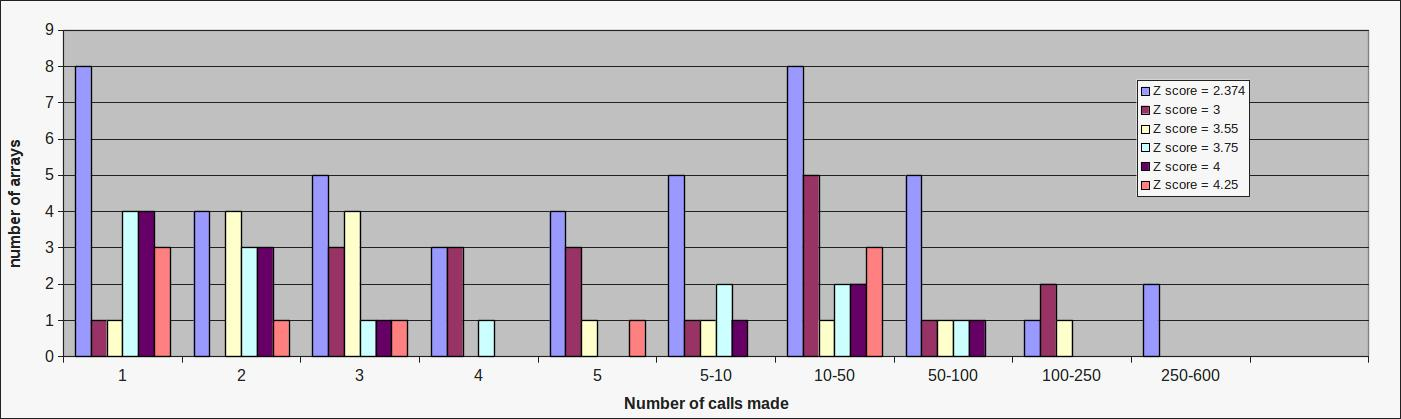
\includegraphics[width=1\linewidth]{./Figures/prospectivesamplecalls}
\caption{Prospective cases: The number of calls per array across a range of threshold in 121 prospective cases}
\label{fig:prospectivesamplecalls}
\end{figure}

\paragraph*{}
It is impossible to know if any of these are actually true positives.

\paragraph*{}
The average size of each call is just over three probes (Table \ref{tab:prosepectivecalls})

\begin{table}[]
\centering
\caption[Prospective cases: The number and size of calls]{Prospective cases: The average and maximum number of probes within a call during analysis of 121 prospective arrays.}
\label{tab:prosepectivecalls}
\resizebox{\textwidth}{!}{%
\begin{tabular}{@{}|l|l|l|l|@{}}
\hline
Z score & Average probes in call & Maximum probes in call & Number of calls \\ \hline
2.374   & 3.24                   & 8                      & 1760            \\ \hline
3       & 3.19                   & 7                      & 591             \\ \hline
3.55    & 3.14                   & 6                      & 246             \\ \hline
3.75    & 3.13                   & 6                      & 180             \\ \hline
4       & 3.1                    & 5                      & 125             \\ \hline
4.25    & 3.09                   & 5                      & 90              \\ \hline
\end{tabular}%
}
\end{table}

\section{Performance of SID}
When uploading a run of 96 arrays, initially each array is processed in approximately two minutes. However, due to the increasingly large features table, the time taken to process an array can increase to around 15 minutes.